\Problem{Ice Archer and Cadillac Crash Setup}{\IceCadSetup}{
For each part of this activity, prepare a pictorial representation, but do not solve the problem (yet).
\begin{itemize}
	\item Draw pictures of ``before'' and ``after.''
	\item Define symbols relevant to the problem.
	\item List known information, and identify the desired unknown.
\end{itemize}
}
\ProblemSub{\IceCadSetupA}{

(a) A 50 kg archer, standing on frictionless ice, shoots a 100 g arrow at a speed of 100 m/s. What is the recoil speed of the archer?
}
\Solution{\IceCadSetupASol}{

\begin{figure}[h]
	\centering
	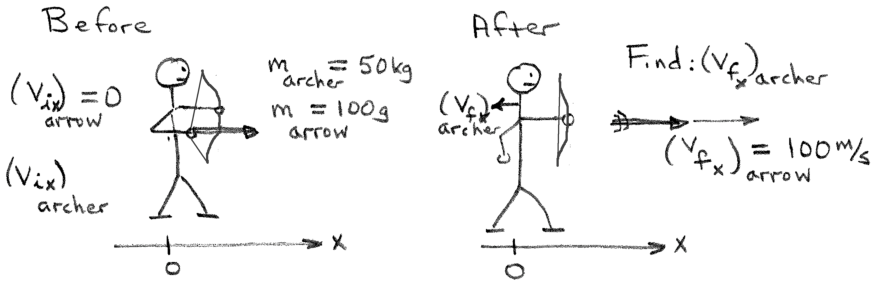
\includegraphics[scale=0.7]{\FileDepth/Activities/Ice_Archer_and_Cadillac_Crash/Archer_on_Ice.pdf}
\end{figure}
}
\ProblemSub{\IceCadSetupB}{

(b) The parking brake on a 2000 kg Cadillac has failed, and it is rolling slowly, at 1 mph, toward a group of small, innocent children. As you see the situation, you realize there is just time for you to drive your 1000 kg Volkswagen head-on into the Cadillac and thus save the children. With what speed should you impact the Cadillac to bring it to a halt?
}
\Solution{\IceCadSetupBSol}{

\begin{figure}[h]
	\centering
	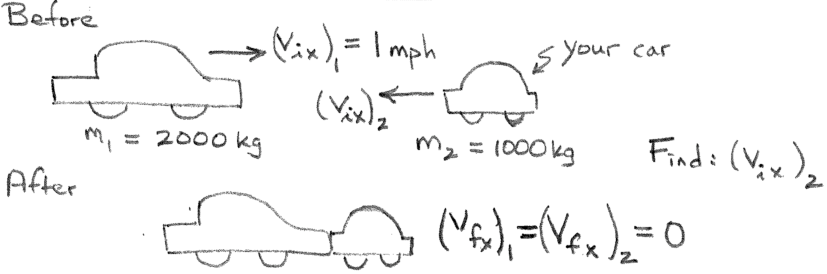
\includegraphics[scale=0.7]{\FileDepth/Activities/Ice_Archer_and_Cadillac_Crash/Cadillac_Collision.pdf}
\end{figure}
}
\Problem{Ice Archer and Cadillac Crash Calculations}{\IceCadCalc}{
Using the setups from the previous activity, solve the following problems.
}
\ProblemSub{\IceCadCalcA}{

(a) A 50 kg archer, standing on frictionless ice, shoots a 100 g arrow at a speed of 100 m/s. What is the recoil speed of the archer?
}
\Solution{\IceCadCalcASol}{

The archer-arrow system conserves momentum, so the combined initial momentum of the pair (which is zero, since they both start from rest) is equal to the combined final momentum of the pair:
\[
\begin{split}
	m_{archer}\cancel{(v_{ix})}_{archer} + m_{arrow}\cancel{(v_{ix})}_{arrow} & = m_{archer}(v_{fx})_{archer} + m_{arrow}(v_{fx})_{arrow} \\
	0 & = m_{archer}(v_{fx})_{archer} + m_{arrow}(v_{fx})_{arrow} \\
	(v_{fx})_{archer} & = -\frac{m_{arrow}}{m_{archer}}(v_{fx})_{arrow} \\
	& = -\frac{0.1\text{ kg}}{50\text{ kg}}(100\text{ m/s}) \\
	& = - 0.2\text{ m/s}.
\end{split}
\]
The archer's recoil speed is 0.2 m/s.
}
\ProblemSub{\IceCadCalcB}{

(b) The parking brake on a 2000 kg Cadillac has failed, and it is rolling slowly, at 1 mph, toward a group of small, innocent children. As you see the situation, you realize there is just time for you to drive your 1000 kg Volkswagen head-on into the Cadillac and thus save the children. With what speed should you impact the Cadillac to bring it to a halt?
}
\Solution{\IceCadCalcBSol}{

The Cadillac-Volkswagen system conserves momentum, so the combined initial momentum of the pair is equal to the combined final momentum of the pair (which is zero, since they crash to a dead stop):
\[
\begin{split}
	m_{1}(v_{ix})_{1} + m_{2}(v_{ix})_{2} & = m_{1}\cancel{(v_{fx})}_{1} + m_{2}\cancel{(v_{fx})}_{1} \\
	m_{1}(v_{ix})_{1} + m_{2}(v_{ix})_{2} & = 0 \\
	(v_{ix})_{2} & = -\frac{m_{1}}{m_{2}}(v_{ix})_{1} \\
	& = -\frac{2000\text{ kg}}{1000\text{ kg}}(1\text{ mph}) \\
	& = - 2\text{ mph}.
\end{split}
\]
You must hit the Cadillac at 2 mph to stop it.
}